\chapter{General Setup}\label{ch:general_setup}

This chapter describes the implementation of the offloading framework in use. However, since this thesis conducts experiments both in simulation and on real robot, there are technical differences between the actual software setups. To avoid redundancies, this chapter introduces the general offloading setup in \cref{sec:general_setup:implementation} that is mutually adopted by the two setups. Furthermore, \cref{sec:general_setup:offloading_strategies} also describes the algorithms that are used to realize different offloading strategies. 
Finally, in \cref{sec:general_setup:evaluation}, this chapter discusses the evaluation paradigm in use for different evaluation metrics.

\section{Implementation}\label{sec:general_setup:implementation}

This thesis implements an offloading pipeline for a robotic object detection task. This includes an offloading module making decision whether to offloading the image from the camera sensor to the edge computer or to compute the image locally using onboard resources. An inference pipeline for object detection task is implemented using pre-trained models from YOLOv5 \cite{Jocher2020} deployed using PyTorch library \cite{Paszke2019}. Furthermore, in order to test the offloading framework in repeatable and comparable experiments, a simulation scenario is implemented in \gls{gazebo} \cite{Koenig2004} and a recording of the scenario run is created with \gls{ros}. Finally, since the output of the object detection task is not used in any downstream applications. This thesis considers and implements various evaluation paradigms to retrieve meaningful results from the data collected during the experiments. To delimit, this thesis only investigates the scenario where one \gls{amr} offloads to one edge computer. Investigations for multi-robot multi-edge scenarios are beyond the scope of this thesis. 

\subsection{Offloading Module}

\begin{figure}[htp]
    \centering
    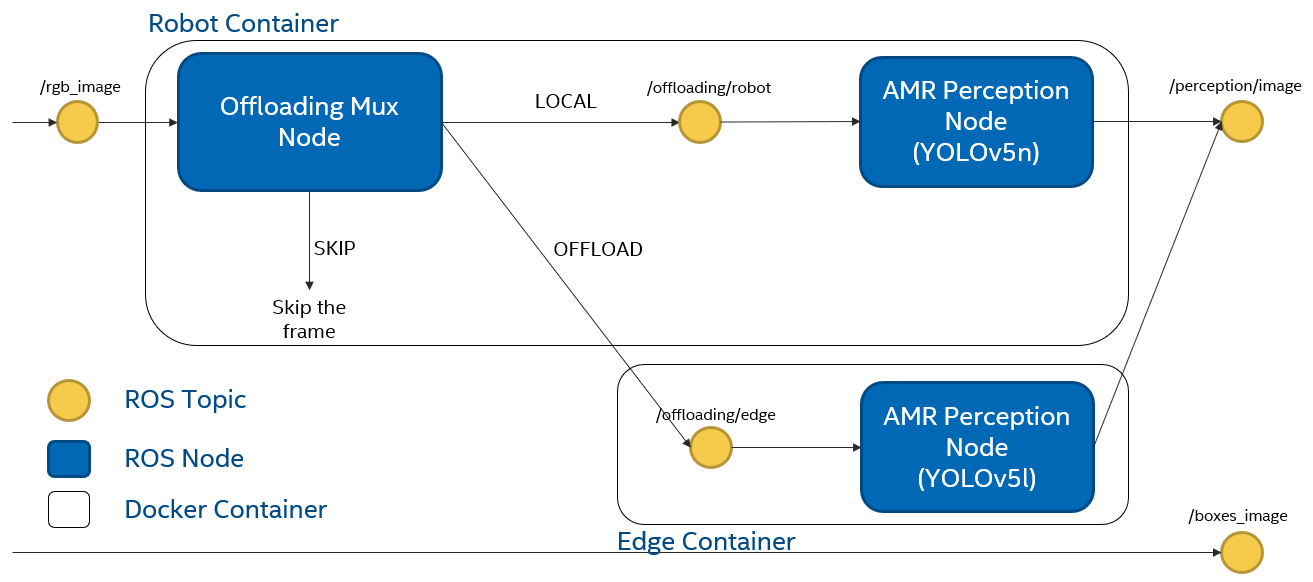
\includegraphics[width=120mm]{figures/setup/general_setup.png}
    \caption{General Setup (TODO: adapt this image)}
    \label{fig:general_setup}
\end{figure}

% TODO: this may need some adaptions to the dynamic offloading module
An offloading pipeline should have the abilities to make decision, coordinate the resources and communicate over the network. A generic offloading pipeline is illustrated in~\cref{fig:general_setup}. Each blue block represents a \gls{ros} node and each yellow circle represents a \gls{ros} topic. The arrows indicate the directions of the data flow. The dotted lines are the virtualization of the robotic system and the edge computer. The images can come from either a camera sensor or the replay of the simulation scenario. Once the \gls{amr} receives the image, the offloading module will have to decide whether to offload the image to the edge computer or pass it to the local perception node, which uses a simpler and lighter model for image inference. The offloading module decides whether to offloads to the edge computer or to compute it locally by publishing the received image to pre-defined \gls{ros} topics. Once the perception nodes receive the image, they will start to do inference on the given image. Then, the processed results are published to another pre-defined \gls{ros} topic and recorded by the \gls{ros} bag. Meanwhile, the ground truth of the simulation for the object detection task is also published to a \gls{ros} topic and recorded by the \gls{ros} bag. 

In order to evaluate different offloading strategies, the offloading module possesses the ability to switch between them. Therefore, the offloading strategies act as plugins for the offloading module. Furthermore, the offloading module is responsible for loading the static hyper-parameters for the offloading strategies on start-up and also for keeping track of the run-time states of the system to allow dynamic offloading strategies. In an offloading pipeline, the system states come from various \gls{ros} nodes observing different functionalities of the system. This information is published to different \gls{ros} topics and subscribed by the offloading module. To reduce the influence of the fluctuation in the observed system states, the offloading module applies a \gls{sma} algorithm to smooth the data. 

Since the offloading pipeline is built upon the \gls{ros}, the behaviour of \gls{ros} and its underlying technical realization is crucial to the behaviour of the offloading pipeline, such as \gls{dds} and \gls{qos} settings. The exact influence of these settings on the behaviour of the offloading pipeline and the performance of the offloading will be discusses in \cref{ch:simulation} and \cref{ch:real_robot_experiment}. 

\subsection{Perception Module}

% discuss the choice of synchronous inference and asynchronous inference. Also defend not retraining the model.

% TODO: find the quote on the edge computers
In general, an offloading task can be any computationally intensive algorithms the \gls{amr} is required to run, such as perception, navigation, \gls{slam}, path planning, etc. This thesis chooses an object detection task as an example, because an object detection task can have significant performance difference between the \gls{amr}'s onboard system and the edge computer, which corresponds to the usage scenario of the edge offloading. An \gls{amr} is usually equipped with a simple onboard system with only access to \gls{cpu}, while an edge computers are usually cloudlets and data centers on premise with access to \gls{gpu}. As mentioned in \cref{ch:background}, the \glspl{amr} use primarily \glspl{dnn} to detect objects. With frameworks like PyTorch that can make use of the \gls{gpu}, the performance difference between \gls{amr}'s onboard system and the edge computer is immense. Therefore, this thesis chooses the object detection as an example for offloading tasks. 

\subsection{State Monitor}

\section{Offloading Strategies}\label{sec:general_setup:offloading_strategies}

\subsection{Implementation within Offloading Module}

% This sections describes how the offloading module resides within the offloading module described in previous section. Also, how the strategies get the static parameters and run-time parameters from the offloading module and static parameter files

\subsection{Static Offloading Strategy}

% This sections describes how RobotOnlyStrategy, EdgeOnlyStrategy, RatioStrategy are implemented. Include a psuedo algorithms here for RatioStrategy

\subsection{Dynamic Offloading Strategy}

\section{Simulation}\label{sec:general_setup:simulation}

\subsection{Environment}

% include a bird-view shot for the simulation with warehouse, robot, and human obstacles in the view.

\subsection{Robot}

% describes how the robot is navigated, describes 

\subsection{Record and Replay}

% describes how the ROS bag is recorded and how is it replayed during the experiments and explain why this is needed. 

\section{Evaluation}\label{sec:general_setup:evaluation}

\subsection{Metrics}

% This sections lists all the evaluation metrics are used and how are they recorded and what tools are used in order to record them. 

\subsection{Synchronous Evaluation Paradigm}

\begin{figure}[htp]
    \centering
    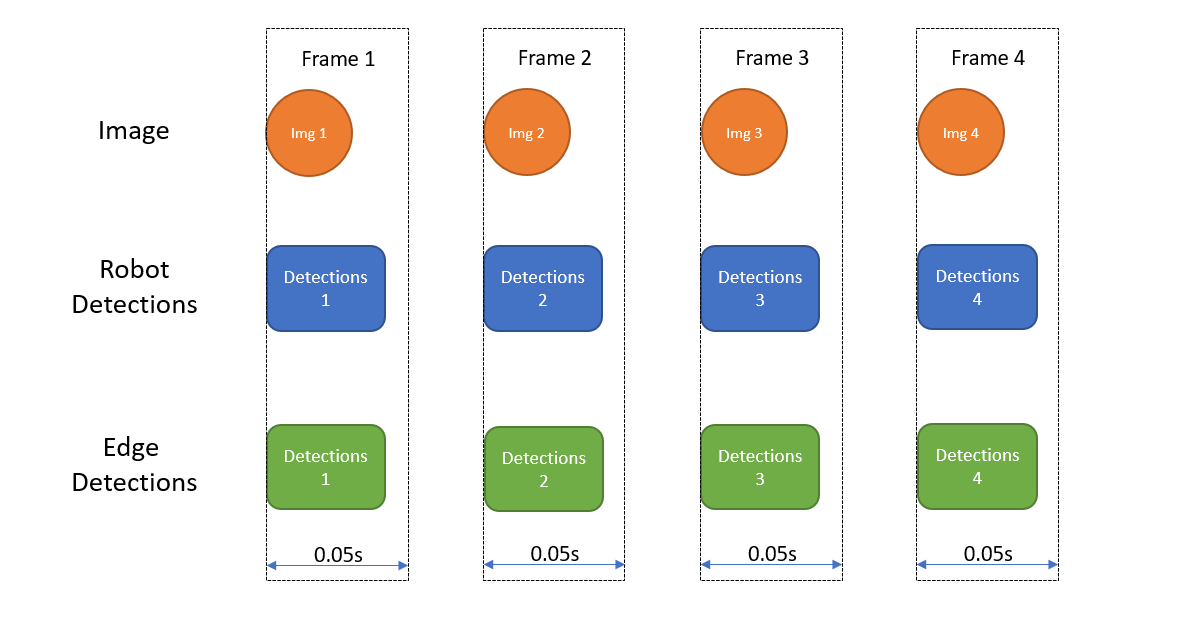
\includegraphics[width=120mm]{figures/setup/sync_eval.png}
    \caption{Synchronous evaluation paradigm}
    \label{fig:sync_eval}
\end{figure}

\subsection{Asynchronous Evaluation Paradigm}

\begin{figure}[htp]
    \centering
    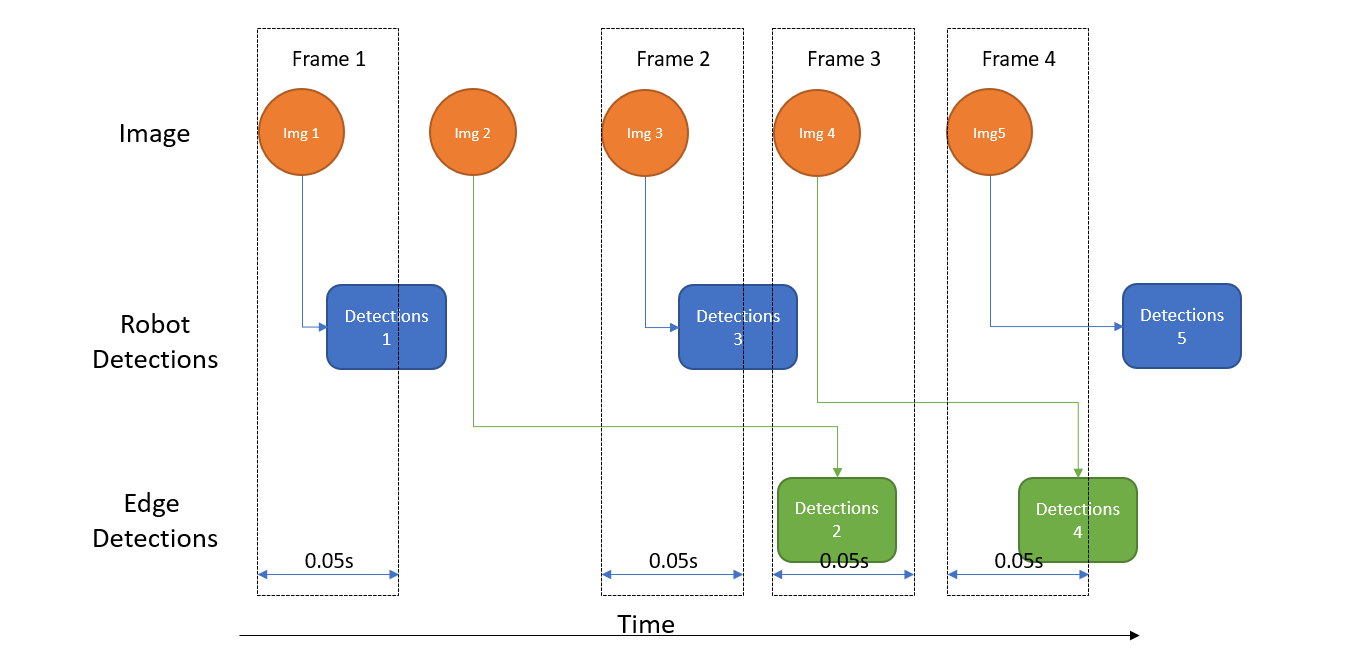
\includegraphics[width=120mm]{figures/setup/async_eval.png}
    \caption{Asynchronous evaluation paradigm}
    \label{fig:async_eval}
\end{figure}

\subsection{Discussion on Evaluation Paradigm}
